Many cryptographic algorithms are considered unbreakable, regardless of the amount of computing power available;
the theoretical security of such algorithms however does not always translate to real-world secure implementations.\\
Regardless of the means of the implementation, the electronic devices that run these cryptosystems often
\textit{leak} information about the internal state of the device, potentially exposing secrets.
But how does a device leak information?

A \textit{side channel} is some observable aspect of a cryptosystem that reveals information held within that system~\cite{DBLP:conf/crypto/Kocher96, DBLP:books/sp/10/Standaert10};
example of side channels can be the execution time of an algorithm, the power consumption of a device or the electromagnetic
radiation emitted while running some operations.\\
In this chapter we will describe the most common side channel attacks, how they can be used to retrieve secret information and
how to mitigate them.

\subsection{Timing attacks}
In a timing attack, the attacker tries to infer information about a secret by measuring the time it takes to execute some operation:
the idea behind this attack is that the time it takes to execute an operation depends on the input of the operation, and thus
by measuring the execution time of the operation we can infer information about the input.

\begin{example}[Unlock the vault]
    Let us consider a simple example: we have a vault with a combination lock, and we want to unlock it. The function
    that checks if the combination entered by the user is correct is shown in the following listing:

    \begin{lstlisting}[language=C, caption={A non constant-time password checker}, label={lst:nonct_pwd}]
    int check_pin(int *pin) {
        int correct_pin[4] = {3, 1, 4, 2};

        for (int i = 0; i < 4; i++) {
            if (pin[i] != correct_pin[i]) {
                return 0;
            }
        }
        return 1;
    }
    \end{lstlisting}
    
    The function simply checks if the PIN entered by the user is equal to the correct PIN, and returns 1 if it is correct and 0 otherwise.
    Being the PIN composed of decimal digits, the total amount of combinations is $10^4$, so on average we would need 5000 guesses to find
    the correct PIN; however, we can reduce the number of guesses needed to find the correct PIN by using a timing attack.

    We can observe that the function returns as soon as a digit of the PIN is incorrect: under the reasonable assumption that we can measure 
    the execution time of the function, we can guess the correct PIN one digit at a time.
    Starting from 0000, we cycle through all the possibilities for the first digit $(0000, 1000, \cdots, 9000)$ and measure the execution time:
    out of the 10 measurements, the one with the highest execution time corresponds to the correct digit; we can then repeat the same process
    for the remaining digits, so that after at most 40 guesses we find the correct pin.
\end{example}

Even though this attack strategy may seem trivial and easy to mitigate, it can still wreck havoc: real-life examples of timing attacks include, 
for example, Spectre~\cite{DBLP:journals/cacm/KocherHFGGHHLMP20} and Meltdown~\cite{DBLP:journals/cacm/LippSGPHHMKGYHS20}, which affects almost 
all modern processors and allowed an attacker to read the memory of any process running on the same machine. Moreover, these attacks do not
necessarily require the attacker to have physical access to the device as they can be performed remotely, as shown in~\cite{DBLP:journals/cn/BrumleyB05, DBLP:conf/esorics/BrumleyT11}.

\subsection{Power attacks}
In order to carry out operations, digital devices require to be powered: the power consumption of a device is usually not fixed, as it can fluctuate
based on a variety of factors. The vast majority of digital devices employs transistors, which act as switches that can be turned on or off; the input
to a transistor can be thought of as a small capacitor and, as such, follows its characteristic equation:
\begin{equation*}
    I = C \cdot \frac{dV}{dt}
\end{equation*}
where $I$ is the current, $C$ is the capacitance of the capacitor and $V$ is the voltage across the capacitor. To turn on a transistor 
(\textit{i.e.} to increase the voltage across the capacitor) we need to apply a \emph{charge} to it: because of this behavior, if we have a changing
voltage on the capacitor, for example when transitioning from 0 to 1, we can observe the flow of current through the capacitor. \\
All operations in a digital circuit are performed by switching millions of transistors on and off: this means that the power consumption
of a digital device is affected by the operations it performs, and thus can be used to infer information about the internal state of the device.

\begin{example}[RSA Square and Multiply]
    The Rivest-Shamir-Adleman (RSA) cryptosystem is one of the most known public-key cryptosystem. In the encryption phase, RSA produces 
    the ciphertext $c$ by raising the plaintext $m$ to the power of the private key $e$ modulo $n$, as shown in the following listing:

    \begin{lstlisting}[language=C, caption={RSA square and multiply}, label={lst:rsa_squaremult}]
    int square_and_multiply(int ptx, int exponent, int modulus) {
        int result = 1;
        while (exponent > 0) {
            if (exponent % 2 == 1) {
                result = (result * ptx) % modulus;
            }
            exponent = exponent / 2;
            ptx = (ptx * ptx) % modulus;
        }
        return result;
    }
    \end{lstlisting}

    The if statement at line 4 determines the execution flow based on the bits of the secret exponent: if the current
    bit is 1 the result is multiplied by the plaintext (\textit{multiply}), otherwise it is not, and we only
    \emph{square} the plaintext.\\
    \begin{figure}[H]
        \caption{Power consumption of the RSA Square and Multiply algorithm}
        \centering
        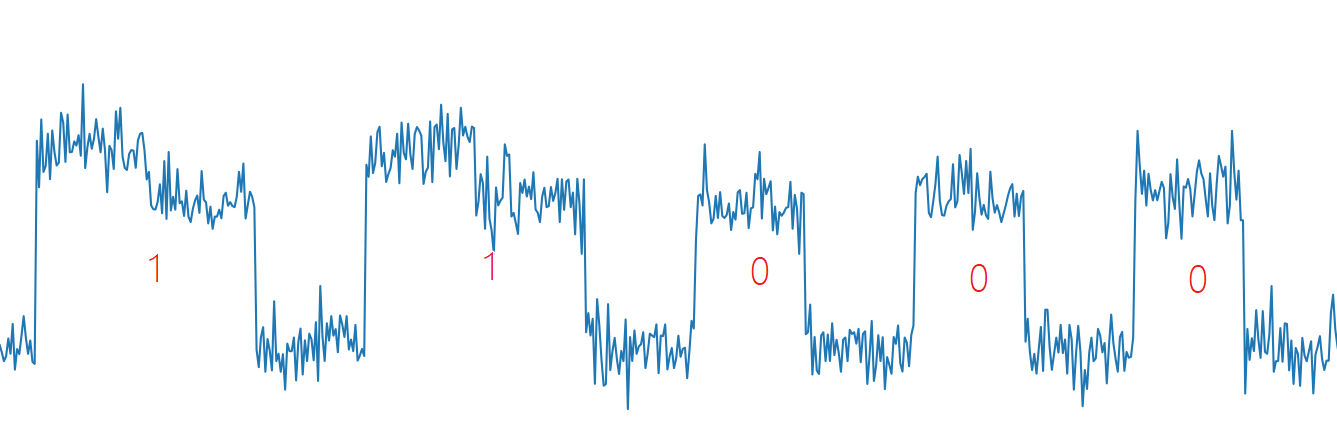
\includegraphics[scale=0.3]{figures/rsa_squaremult.png}
        \label{fig:rsa_squaremult}
    \end{figure}
    As shown in the figure above, by looking at the power consumption we can clearly distinguish whether the exponent
    bit is 1 or 0, and thus we can infer the value of the secret exponent.
\end{example}

\subsubsection{Measurements and attacks}
    When it comes to actually measuring the power consumption of a device we have two main approaches:
    \begin{itemize}
        \item Measure the voltage across a \emph{shunt resistor}: a resistor with a fixed value is placed between the power source
        and the device
        \item Measure the emitted electromagnetic radiation: the current flowing through the device induces magnetic field in the wires, that
        we can pick up with a near-field probe
    \end{itemize}
    Both methods have their pros and cons: the first one is more accurate, but requires to phisically install the shunt resistor on the device;
    the second one is non-intrusive, but the measurements are tipically noisy due to external interferences.

    Regardless of the source of a power trace, there are several possibilities to carry out an attack~\cite{DBLP:journals/cryptography/RandolphD20}, such as:
    \begin{itemize}
        \item Simple Power Analysis: observe the power consumption over a single trace
        \item Differential Power Analysis~\cite{DBLP:conf/crypto/KocherJJ99}: analyze multiple executions over the same algorithm with different inputs to detect small input-dependent differences
        \item Template attacks~\cite{DBLP:conf/ches/ChariRR02}: collect a large number of traces and use them to build a \emph{template} of the power consumption of the device to detect
        when the device is performing a specific operation 
    \end{itemize}

\subsection{Countermeasures}
    The existence of a side-channel does not necessarily mean that an attack is possible: in fact, there are a number of countermeasures
    that can mitigate the risk of a successful attack.

    Regarding timing attacks, the most common countermeasure is to use \emph{constant-time} algorithms, that take the same amount of time to
    execute regardless of the input; this can be achieved, for example, by replacing branching statements that depend on the inputs.

    A very effective way to avoid leakage, especially with respect to power attacks, is to randomize the inputs of the algorithm without
    affecting the output. To do so, we can \emph{mask} the inputs: the basic principle of masking~\cite{DBLP:conf/eurocrypt/ProuffR13} is to split every sensitive value $x$ 
    into $d+1$ \textit{shares}, in such a way that the following relation holds:
    \begin{equation}
        x = x_0 \odot x_1 \odot \cdots \odot x_d
    \end{equation}
    The shares $x_1, \cdots, x_d$ are called \textit{masks} and are randomly sampled, while the secret $x_0$ is processed in 
    such a way that the relation above holds. The goal of masking is to make the sensitive value indistinguishable from
    a random value, so that the observation of a side channel does not reveal any sensitive information, but only random noise.
    There is no particular constraint on the choice of the operation $\odot$ as long as it preserves the relation above;
    in practice, the most common choice is to use the XOR operation, as it is very fast and easy to implement: such a masking
    scheme (e.g.~\cite{DBLP:conf/crypto/IshaiSW03}) is often referred to as \emph{boolean} masking.
    As proven in~\cite{DBLP:conf/crypto/ChariJRR99}, a masking scheme with $d$ shares is a sound counermeasure against a side-channel attack 
    of $d$-th order, where an attacker can have up to $d$ \emph{probes} on the target system; this means that a $d+1$-th order
    attack could be possible, but such attacks become impractical as $d$ increases.

